\documentclass[xcolor=table]{beamer}
\usetheme{Rochester}
\usepackage{amsmath}
\usepackage{amssymb}
\usepackage{graphicx}
\usepackage{tikz}
\usepackage{pgfplots}
\pgfplotsset{compat=1.18}
\usetikzlibrary{arrows.meta}
\usetikzlibrary{calc}
\usetikzlibrary{decorations.pathmorphing}
\newcommand*\circled[1]{\tikz[baseline=(char.base)]{
            \node[shape=circle,draw, minimum size=3.5mm,inner sep=0.5pt] (char) {#1};}}

\usepackage{ifthen}
\usepackage[noend]{algpseudocode}
\usepackage{soul}
\usepackage{isabelle}
\usepackage{isabellesym}
\isabellestyle{it}

\DeclareMathOperator{\mbind}{\text{\isa{\isasymbind}}}
\DeclareMathOperator{\expect}{\mathrm{E}}

\renewcommand{\algorithmicrequire}{\textbf{Input:}}
\renewcommand{\algorithmicensure}{\textbf{Output:}}
\newcommand{\ift}[3]{\mathbf{if} \; #1 \; \mathbf{then} \; #2 \; \mathbf{else} \; #3}
\newcommand{\integral}[3]{\int_{#1} \! #2 \, \mathrm{d} #3}

\newcommand{\getsr}{\xleftarrow{\$}}

\title{Verification of the CVM algorithm with a Functional Probabilistic Invariant}
\author{E. Karayel\inst{1}, J. Watt\inst{2}, D. Khu\inst{2}, K. Meel\inst{4,5}, Y. K. Tan\inst{2,3}}
\institute[VFU]{
  \inst{1}%
    Technical University of Munich, Germany
  \and
  \inst{2}%
    Institute for Infocomm Research (I$^2$R), A*STAR, Singapore
  \and
  \inst{3}%
    Nanyang Technological University, Singapore
  \and
  \inst{4}%
    Georgia Institute of Technology, Atlanta, GA, USA
  \and
  \inst{5}%
    University of Toronto, Canada
}

\usepackage{mathtools}
\DeclareMathOperator{\prob}{\mathcal P}
\DeclareMathOperator{\bigo}{\mathcal O}
\DeclarePairedDelimiter{\ceil}{\lceil}{\rceil}
\DeclareMathOperator{\Ber}{\mathrm{Ber}}
\DeclareMathOperator{\indicat}{\mathrm{I}}

\begin{document}
\AtBeginSection[]
{
    \begin{frame}
        \frametitle{Table of Contents}
        \tableofcontents[currentsection]
    \end{frame}
}

\frame{\titlepage}
\begin{frame}
\frametitle{Table of Contents}
\tableofcontents
\end{frame}

\section{Introduction to the CVM algorithm}
\begin{frame}
\frametitle{What is the CVM algorithm?}
\begin{itemize}
\item Name after initals of S. Chakraborty, N. V. Vinodchandran, K. S. Meel
\pause
\item Streaming Algorithm (one sequential pass): $a_1, \ldots, a_l$
\pause
\item Algorithm has only limited mutable state: $\bigo( \varepsilon^{-2} \ln(\delta^{-1} l ) b )$
\pause
\item Approximation of the count of distinct elements
\pause
\item Randomized
\pause
\item Small error with high probability
\[
  \prob\left(|X - |A|| \geq \varepsilon |A| \right) \leq \delta 
\]
for choosable $\varepsilon > 0$, $\delta > 0$
\pause
\item Suprisingly simple compared to previous algorithms for the same problem \pause (see e.g. article in Quanta Magazine\cite{quanta})
\pause
\item No hashing
\end{itemize}
\end{frame}
\begin{frame}
\frametitle{Illustration of Streaming Algorithms}
\begin{figure}
\begin{center}
\begin{tikzpicture}[
  streamcell/.style={rectangle, draw=black, fill=black!15, thick, text centered,inner sep=3pt,minimum width=0.6cm},
]
\node[streamcell] (cell1) at (-3,2) {$a_1$};
\node[streamcell] (cell1) at (-2.4,2) {$a_1$};
\node[streamcell] (cell1) at (-1.8,2) {$a_2$};
\node at (0,2) {$\cdots$};
\node[streamcell] (cell1) at (2,2) {$a_{l}$};
\node (robot) at (0,0)
    {\includegraphics[width=.25\textwidth]{contrib/vecteezy_cute-robot-holding-clipboard-cartoon-icon-illustration_53779545_655/vecteezy_cute-robot-holding-clipboard-cartoon-icon-illustration_53779545}};
\end{tikzpicture}
\end{center}
\end{figure}
\end{frame}

\begin{frame}[label=cvm_algorithm]
\frametitle{The CVM Algorithm}
\begin{algorithmic}
  \Require Stream elements $a_1,\dots,a_l$, $0 < \varepsilon$, $0 < \delta < 1$.
  \Ensure A cardinality estimate $R$ for set $A = \{ a_1,\dots,a_l \}$ % such that $\prob \left( |R - |A| | > \varepsilon |A| \right) \leq \delta$
  \State $\chi \gets \{\}, p \gets 1, n = \ceil*{\frac{12}{\varepsilon^2} \ln{(\frac{6l}{\delta})} }$
  \For{$i \gets 1$ to $l$}
    \State $b \getsr \Ber(p)$ \Comment random bit $b$ from the Bernoulli distribution
    \If{$b$} \Comment insert $a_i$ if $b$ is true (with prob. $p$)
      \State $\chi \gets \chi \cup \{a_i\}$
    \Else \Comment remove $a_i$ otherwise
      \State $\chi \gets \chi - \{a_i\}$
    \EndIf
    \If{$|\chi| = n$} \Comment subsample if buffer $\chi$ is full
      \State $\chi \getsr \mathrm{subsample}(\chi)$
      \State $p \gets \frac{p}{2}$
    \EndIf
    \If{$|\chi| = n$}
      \Return $\bot$ \Comment fail if $\chi$ remains full
    \EndIf
  \EndFor
  \State \Return $\frac{|\chi|}{p}$ \Comment estimate cardinality of $A$
\end{algorithmic}
\end{frame}

\definecolor{streamcolor1}{rgb}{1.0, 0.94, 0.0}
\definecolor{streamcolor2}{rgb}{0.9, 0.17, 0.31}
\definecolor{streamcolor3}{rgb}{0.0, 0.5, 0.0}
\definecolor{streamcolor4}{rgb}{0.0, 0.5, 1.0}
\definecolor{streamcolor5}{rgb}{0.74, 0.2, 0.64}
\definecolor{tailcoinbordercolor}{rgb}{0.13, 0.67, 0.8}
\definecolor{tailcoinfillcolor}{rgb}{0.54, 0.81, 0.94}
\definecolor{headcoinbordercolor}{rgb}{1.0, 0.44, 0.37}
\definecolor{headcoinfillcolor}{rgb}{0.98, 0.91, 0.71}

\newcommand{\illustratestate}[7]{
  \begin{tikzpicture}[
    streamcell/.style={circle, draw=black, fill=black!15, thick, text centered,inner sep=3pt,minimum width=0.6cm},
    arrow/.style={thick,-{Latex[length=.32cm, width=.32cm,fill=white]}},
    coin/.style={circle, draw=orange, fill=yellow, thick},
  ]
  \node[streamcell,fill=streamcolor3] at (0cm,0 cm) {};
  \node[streamcell,fill=streamcolor1] at (1cm,0 cm) {};
  \node[streamcell,fill=streamcolor3] at (2cm,0 cm) {};
  \node[streamcell,fill=streamcolor2] at (3cm,0 cm) {};
  \node[streamcell,fill=streamcolor4] at (4cm,0 cm) {};
  \node[streamcell,fill=streamcolor5] at (5cm,0 cm) {};
  \node[streamcell,fill=streamcolor1] at (6cm,0 cm) {};
  \node[streamcell,fill=streamcolor2] at (7cm,0 cm) {};
  \node[streamcell,fill=streamcolor3] at (8cm,0 cm) {};
  \node at (9cm,0cm) {$\cdots$};
  \draw[arrow] (1cm * #1, -1.5cm) to (1cm * #1, -0.5cm);
  \node (robot) at (0,-3.5cm){\robot{.25\textwidth}};

  \node[anchor=west] at (1.4cm, -3.1cm) {$\chi = \{$};
  \ifthenelse{\equal{#3}{empty}}{}{\node[streamcell,fill=#3] at (3cm, -3.1cm) {};}
  \ifthenelse{\equal{#4}{empty}}{}{\node[streamcell,fill=#4] at (3.8cm, -3.1cm) {};}
  \ifthenelse{\equal{#5}{empty}}{}{\node[streamcell,fill=#5] at (4.6cm, -3.1cm) {};}
  \ifthenelse{\equal{#6}{empty}}{}{\node[streamcell,fill=#6] at (5.4cm, -3.1cm) {};}
  \node at (6cm, -3.1cm) {$\}$};

  \ifthenelse{\equal{#7}{head}}{
    \node[coin,fill=headcoinfillcolor,draw=headcoinbordercolor] at (-1cm,-3.5cm) {H}; 
  }{}
  \ifthenelse{\equal{#7}{tail}}{
    \node[coin,fill=tailcoinfillcolor,draw=tailcoinbordercolor] at (-1cm,-3.5cm) {T}; 
  }{}

  \node[anchor=west] at (1.4cm, -3.8cm) {$p = #2, n = 4$};

  \end{tikzpicture}
}

\begin{frame}
\frametitle{Illustration of the Algorithm}

\only<1>{\illustratestate{0}{1}{empty}{empty}{empty}{empty}{none}}
\only<2>{\illustratestate{0}{1}{empty}{empty}{empty}{empty}{head}}
\only<3>{\illustratestate{0}{1}{streamcolor3}{empty}{empty}{empty}{head}}
\only<4>{\illustratestate{1}{1}{streamcolor3}{empty}{empty}{empty}{head}}
\only<5>{\illustratestate{2}{1}{streamcolor3}{streamcolor1}{empty}{empty}{head}}
\only<6>{\illustratestate{3}{1}{streamcolor3}{streamcolor1}{empty}{empty}{head}}
\only<7>{\illustratestate{4}{1}{streamcolor3}{streamcolor1}{streamcolor2}{empty}{head}}
\only<8>{\illustratestate{4}{1}{streamcolor3}{streamcolor1}{streamcolor2}{streamcolor4}{head}}
\only<9>{\illustratestate{4}{1}{empty}{streamcolor1}{streamcolor2}{empty}{none}}
\only<10>{\illustratestate{4}{\frac{1}{2}}{empty}{streamcolor1}{streamcolor2}{empty}{none}}
\only<11>{\illustratestate{5}{\frac{1}{2}}{empty}{streamcolor1}{streamcolor2}{empty}{none}}
\only<12>{\illustratestate{5}{\frac{1}{2}}{empty}{streamcolor1}{streamcolor2}{empty}{head}}
\only<13>{\illustratestate{5}{\frac{1}{2}}{streamcolor5}{streamcolor1}{streamcolor2}{empty}{head}}
\only<14>{\illustratestate{6}{\frac{1}{2}}{streamcolor5}{streamcolor1}{streamcolor2}{empty}{none}}
\only<15>{\illustratestate{6}{\frac{1}{2}}{streamcolor5}{streamcolor1}{streamcolor2}{empty}{tail}}
\only<16>{\illustratestate{6}{\frac{1}{2}}{streamcolor5}{empty}{streamcolor2}{empty}{taiil}}
\only<17>{\illustratestate{7}{\frac{1}{2}}{streamcolor5}{empty}{streamcolor2}{empty}{taiil}}
\end{frame}


\againframe{cvm_algorithm}

\begin{frame}
\frametitle{Comparison with Previous Algorithms}
\alt<2>{\definecolor{colorrowa}{rgb}{0,0.8,0.6}}{\definecolor{colorrowa}{rgb}{1,1,1}}
\alt<3>{\definecolor{colorrowb}{rgb}{0,0.8,0.6}}{\definecolor{colorrowb}{rgb}{1,1,1}}
\alt<4>{\definecolor{colorrowc}{rgb}{0,0.8,0.6}}{\definecolor{colorrowc}{rgb}{1,1,1}}
\alt<5>{\definecolor{colorrowd}{rgb}{0,0.8,0.6}}{\definecolor{colorrowd}{rgb}{1,1,1}}
\alt<6>{\definecolor{colorrowe}{rgb}{0,0.8,0.6}}{\definecolor{colorrowe}{rgb}{1,1,1}}
\alt<7>{\definecolor{colorrowf}{rgb}{0,0.8,0.6}}{\definecolor{colorrowf}{rgb}{1,1,1}}
\begin{table}
\begin{tabular}{l | l | l | l}
\hline
Year & Author(s) & Space & Remarks \\
\hline
\rowcolor{colorrowa} 2001 & Bar-Yossef et al.~\cite{baryossef2002} & $\tilde{O}( \ln(\delta^{-1}) (\varepsilon^{-2}  + b ))$ &  M. H. \\
\rowcolor{colorrowb} 2007 & HLL~\cite{flajolet2007} &  $O(\ln(\delta^{-1} \varepsilon^{-2} \ln b)$ & O. M. H. \\
\rowcolor{colorrowc} 2010 & Kane et al.~\cite{kane2010} & $O( \ln(\delta^-1) (\varepsilon^{-2} + b) )$ & H. \\
\rowcolor{colorrowd} 2020 & B\l{}asiok~\cite{blasiok2020} & $O( \varepsilon^{-2} \ln (\delta^{-1}) + b )$ & H. E. \\
\rowcolor{colorrowe} 2022 & Karayel~\cite{karayel2022} & $O( \varepsilon^{-2} \ln (\delta^{-1}) + b )$ & H. E. M. \\
\rowcolor{colorrowf} 2023 & Chakraborty et al.~\cite{chakraborty2023} & $O( \varepsilon^{-2} \ln( \delta^{-1} l) b )$ & - \\
\end{tabular}
\end{table}
Abbreviations: 
\begin{itemize}
\item M: Supports merging of sketches.
\item H: Relies on hash functions.
\item E: Relies on expander graphs.
\item O: Random oracle model.
\end{itemize}
\end{frame}

\section{Summary of Results}
\begin{frame}
\frametitle{Summary of Results}
\begin{itemize}
\item <2-> Verification of Correctness \only<6->{using the original and new method}
\item <3-> Discovery of a new more succinct proof\only<6->{ (1003 lines vs.\ 2634 lines)}\only<4->{, which is based on a \emph{new} proof technique for randomized algorithms.}
\item <5-> We call it: \emph{Functional Probabilistic Invariants}
\item <7-> Discovery of an unbiased total variant of the algorithm. (Application of our new technique.)
\end{itemize}
\end{frame}

\section{Verification using Functional Probabilistic Invariants}
\begin{frame}<1-5>[label=algsplit]
\frametitle{Another slide with the algorithm}
\begin{algorithmic}
  \State $\chi \gets \{\}, p \gets 1, n = \ceil*{\frac{12}{\varepsilon^2} \ln{(\frac{\only<6>{3}\only<1-5>{6}l}{\delta})} }$
  \For{$i \gets 1$ to $l$}
    \State $b \getsr \Ber(p)$
    \If{$b$}
      \State $\chi \gets \chi \cup \{a_i\}$
    \Else
      \State $\chi \gets \chi - \{a_i\}$
    \EndIf
    \If{$|\chi| = n$}
      \State $\chi \getsr \only<1-5>{\mathrm{subsample}}\only<6>{\mathrm{subsample'}}(\chi)$
      \State $p \gets \frac{p}{2}$
    \EndIf
    \If{$|\chi| = n$}
      \Return $\bot$
    \EndIf
  \EndFor
  \State \Return $\frac{|\chi|}{p}$
\end{algorithmic}

\tikz[overlay, shift=(current page.north west)]{
\begin{scope}[x={(current page.north east)},y={(current page.south west)}]

\only<2->{
        \fill[blue!50, opacity=0.5] (0.07,0.4) rectangle (0.7,0.67);
        \node [anchor=west] at (0.45,0.535) {Step 1};
}
\only<3->{
        \fill[red!50, opacity=0.5] (0.07,0.675) rectangle (0.7,0.845);
        \node [anchor=west] at (0.45,0.76) {Step 2};
}
\only<4->{
        \draw[thick, decorate, decoration={snake,amplitude=0.6pt}] (0.072,0.87) -- (0.42, 0.87);
}
\only<6>{
       \fill[white] (0.07,0.846) rectangle (0.7,0.895);
%        \node [anchor=west] at (0.45,0.87) {Step 3};
}
\only<5->{
  \fill[green!50, opacity=0.5] (0.03, 0.895) rectangle (0.7, 0.97);
   \node [anchor=west] at (0.45,0.932) {Estimate};
}
\end{scope}
}
\end{frame}

\begin{frame}
\frametitle{Giry Monad}
We can represent randomized algorithms using the Giry monad:
\begin{itemize}
\item Primitive random operations, e.g., $\Ber(p)$
\item Return operation $\mathrm{return} \, x$
\item Sequential compositon $m \mbind f$
\end{itemize}
\pause
\begin{block}{Fact}
For an event $E$: 
\begin{eqnarray*}
\prob_{m \mbind f}( E )  & = & \int_{m} P_{f(x)} (E) \, dx \onslide<3->{= \sum_x P_{f(x)} (E) P_m({x})} \\
\onslide<4->{\expect_{m \mbind f}[ g ]  & = & \int_{m} \expect_{f(x)} [g] \, dx}
\end{eqnarray*}
\end{block}
\end{frame}

\againframe<5>{algsplit}

\begin{frame}
\frametitle{Our algorithm in monadic notation}
\newcommand{\stepone}{\textcolor{blue}{\mathrm{step}_1}}
\newcommand{\steptwo}{\textcolor{red}{\mathrm{step}_2}}
\newcommand{\estimate}{\textcolor{green}{\mathrm{estimate}}}
\begin{eqnarray*}
  \mathrm{init} & \mbind & \stepone a_1 \mbind \steptwo \mbind \stepone a_2 \mbind \steptwo \cdots \\
  & \mbind & \stepone a_l \mbind \steptwo \mbind \estimate \\
  \mathrm{init} & = & \mathrm{return} \, (1, \emptyset)
\end{eqnarray*}
\pause
Example invariant:
\[
\expect \left[ \frac{\indicat(s \in \chi)}{p} \right]= 1
\]
for all $s$ that are present in the stream.
\end{frame}

\begin{frame}
\frametitle{Verifying the invariant: Induction step for Step 2}
\begin{block}{Assumption}
$\expect_m \left[ \frac{\indicat(s \in \chi)}{p} \right] = 1$
\end{block}
\begin{block}{Goal}
$ L := \expect_{m \mbind \mathrm{step}_2} \left[ \frac{\indicat(s \in \chi)}{p} \right]= 1$
\end{block}
\[
L =
\only<1>{\expect_{m \mbind \mathrm{step}_2} \left[ \frac{\indicat(s \in \chi)}{p} \right]}
\only<2>{\integral{m}
      {\left(\ift{|\chi|=n}{\integral{\mathrm{subs.}(\chi)}{\frac{\indicat(s \in \tau)}{p/2}}{\tau}}{\frac{\indicat(s \in \chi)}{p}} \right)}
      {\sigma}}
\only<3>{\integral{m}
      {\left(\ift{|\chi|=n}{\frac{2}{p}\integral{\mathrm{subs.}(\chi)}{\indicat(s \in \tau)}{\tau}}{\frac{\indicat(s \in \chi)}{p}} \right)}
      {\sigma}}
\only<4>{\integral{m}
      {\left(\ift{|\chi|=n}{\frac{2}{p}\frac{\indicat(s \in \chi)}{2}}{\frac{\indicat(s \in \chi)}{p}} \right)}
      {\sigma}}
\only<5>{\integral{m}
      {\left(\ift{|\chi|=n}{\frac{\indicat(s \in \chi)}{p}}{\frac{\indicat(s \in \chi)}{p}} \right)}
      {\sigma}}
\only<6>{\integral{m}
      {\frac{\indicat(s \in \chi)}{p} }
      {\sigma}}
\only<7>{1}
\]
\end{frame}

\begin{frame}[label=observations]
\frametitle{Observations}
\begin{itemize}
\item Expected result is the count of distinct elements.
\only<2->{\item We want to establish concentration}
\only<4->{\item Can extend the above recursive analysis to more complex expressions: }
\only<5>{
\[
  \expect \left[ h \left( \frac{\indicat(s \in \chi)}{p} \right)\right] \leq h(1)
\]
for every non-negative concave function $h$ and stream elements $s$.}
\only<6->{
\[
  \expect \left[ \prod_{s \in S}  h \left( \frac{\indicat(s \in \chi)}{p} \right)\right] \leq h(1)^{|S|}
\]
for every non-negative concave function $h$ and subset of stream elements $S$.}
\only<7->{\item $\Rightarrow$\only<8->{*} Approximation Guarantee
\[
  \prob\left(|X - |A|| \geq \varepsilon |A| \right) \leq \delta 
\]
\only<8->{\item More details in the paper.}
}
\end{itemize}
\only<3>{
\begin{figure}
\centering
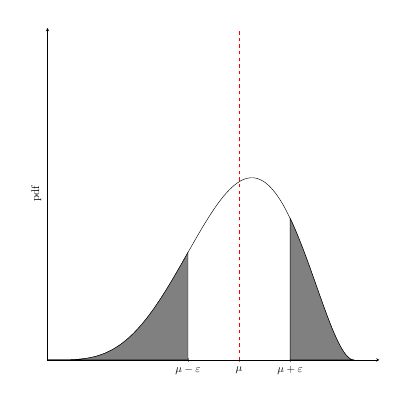
\begin{tikzpicture}[scale=0.4]
\begin{axis}[
    xmin=0, xmax = 6.5,
    ymin=0, ymax=0.7,
    axis lines = left,
    xlabel = {},
    xtick={2.75,3.75,4.75},
    xticklabels={$\mu-\varepsilon$,$\mu$,$\mu+\varepsilon$},
    ytick=\empty,
    ylabel = {pdf},
    height = \textwidth,
    width = \textwidth,
]
\addplot [
    domain=0:6, 
    samples=1000, 
]{max(0,35/2*(x/6)^4*(1-x/6)^2)};
\addplot [
    domain=4.75:6, 
    samples=1000, 
    fill=gray,
]{max(0,35/2*(x/6)^4*(1-x/6)^2)} \closedcycle;
\addplot [
    domain=0:2.75, 
    samples=1000, 
    fill=gray,
]{max(0,35/2*(x/6)^4*(1-x/6)^2)} \closedcycle;
\draw[color=red, dashed] (axis cs:3.75, 0) -- (axis cs:3.75, 0.7);
\end{axis}
\end{tikzpicture}
\begin{tikzpicture}[scale=0.4]
\begin{axis}[
    xmin=0, xmax = 6.5,
    ymin=0, ymax=0.7,
    axis lines = left,
    xlabel = {},
    xtick={2.75,3.75,4.75},
    xticklabels={$\mu-\varepsilon$,$\mu$,$\mu+\varepsilon$},
    ytick=\empty,
    ylabel = {pdf},
    height = \textwidth,
    width = \textwidth,
]
\addplot [
    domain=0:6, 
    samples=1000, 
]{0.65*exp(-(2*(x-3.75))^2)};
\addplot [
    domain=4.75:6, 
    samples=1000, 
    fill=gray,
]{0.65*exp(-(2*(x-3.75))^2)} \closedcycle;
\addplot [
    domain=0:2.75, 
    samples=1000, 
    fill=gray,
]{0.65*exp(-(2*(x-3.75))^2)} \closedcycle;
\draw[color=red, dashed] (axis cs:3.75, 0) -- (axis cs:3.75, 0.7);
\end{axis}
\end{tikzpicture}
\end{figure}
}
\end{frame}

%% \begin{frame}
%% \frametitle{Concentration}
%% \begin{tikzpicture}[scale=0.5]
%% \begin{axis}[
%%     xmin=0, xmax = 6.5,
%%     ymin=0, ymax=0.7,
%%     axis lines = left,
%%     xlabel = {},
%%     xtick={2.75,3.75,4.75},
%%     xticklabels={$\mu-\varepsilon$,$\mu$,$\mu+\varepsilon$},
%%     ytick=\empty,
%%     ylabel = {pdf},
%%     height = \textwidth,
%%     width = \textwidth,
%% ]
%% \addplot [
%%     domain=0:6, 
%%     samples=1000, 
%% ]{max(0,35/2*(x/6)^4*(1-x/6)^2)};
%% \addplot [
%%     domain=4.75:6, 
%%     samples=1000, 
%%     fill=gray,
%% ]{max(0,35/2*(x/6)^4*(1-x/6)^2)} \closedcycle;
%% \addplot [
%%     domain=0:2.75, 
%%     samples=1000, 
%%     fill=gray,
%% ]{max(0,35/2*(x/6)^4*(1-x/6)^2)} \closedcycle;
%% \draw[color=red, dashed] (axis cs:3.75, 0) -- (axis cs:3.75, 0.7);
%% \end{axis}
%% \end{tikzpicture}
%% \begin{tikzpicture}[scale=0.5]
%% \begin{axis}[
%%     xmin=0, xmax = 6.5,
%%     ymin=0, ymax=0.7,
%%     axis lines = left,
%%     xlabel = {},
%%     xtick={2.75,3.75,4.75},
%%     xticklabels={$\mu-\varepsilon$,$\mu$,$\mu+\varepsilon$},
%%     ytick=\empty,
%%     ylabel = {pdf},
%%     height = \textwidth,
%%     width = \textwidth,
%% ]
%% \addplot [
%%     domain=0:6, 
%%     samples=1000, 
%% ]{0.65*exp(-(2*(x-3.75))^2)};
%% \addplot [
%%     domain=4.75:6, 
%%     samples=1000, 
%%     fill=gray,
%% ]{0.65*exp(-(2*(x-3.75))^2)} \closedcycle;
%% \addplot [
%%     domain=0:2.75, 
%%     samples=1000, 
%%     fill=gray,
%% ]{0.65*exp(-(2*(x-3.75))^2)} \closedcycle;
%% \draw[color=red, dashed] (axis cs:3.75, 0) -- (axis cs:3.75, 0.7);
%% \end{axis}
%% \end{tikzpicture}
%% \end{frame}

%% \againframe<2->{observations}

\begin{frame}
\frametitle{Observations II}
\begin{itemize}
\item The new proof is much shorter than the original proof (1003 lines vs. 2634 lines.)
\only<2->{\item \emph{As far as we can tell,} this technique is new.}
\only<3->{\item The new proof opens up the design-space of the algorithm.}
\only<4>{\item For example we can select the subsampling ratio dynamically.}
\only<6->{\item More interestingly: It is possible to use a different subsampling operation.}
\only<7->{\item Select a random $nf$-subset (where $\frac{1}{2} \leq f < 1$, $nf \in \mathbb Z$).}
\only<8->{\item $\Rightarrow$ Unbiased algorithm}
\end{itemize}
\end{frame}
\againframe<5-6>{algsplit}

\section{Sketch of the Original Proof}
\begin{frame}
\frametitle{Original Proof}
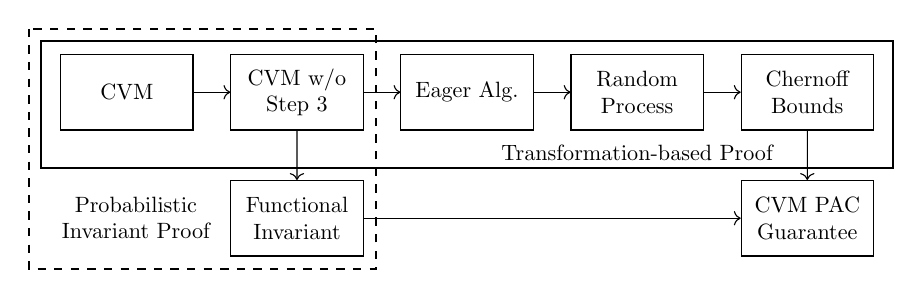
\begin{tikzpicture}[node distance=2.7cm, auto,scale=0.8,every node/.style={scale=0.8}]

    \node (A) [draw, rectangle, minimum width=2.1cm, minimum height=1.2cm, align=center] {CVM};
    \node (B) [draw, rectangle, minimum width=2.1cm, minimum height=1.2cm, align=center, right of=A] {CVM w/o\\ Step 3};
    \node (C) [draw, rectangle, minimum width=2.1cm, minimum height=1.2cm, align=center, right of=B] {Eager Alg.};
    \node (D) [draw, rectangle, minimum width=2.1cm, minimum height=1.2cm, align=center, right of=C] {Random \\ Process};
    \node (E) [draw, rectangle, minimum width=2.1cm, minimum height=1.2cm, align=center, right of=D] {Chernoff \\ Bounds};

    \node (C') [draw, rectangle, minimum width=2.1cm, minimum height=1.2cm, align=center, below of=B, node distance = 2.0cm] {Functional\\Invariant};

    \node (pac) [draw, rectangle, minimum width=2.1cm, minimum height=1.2cm, align=center, below of=E, node distance = 2.0cm] {CVM PAC\\ Guarantee};

    \draw[thick] ($(A.north west) + (-0.3,0.2)$) rectangle ($(E.south east) + (0.3,-0.6)$);
    \node[anchor=south] at ($(D.south) + (0.0,-0.6)$) {Transformation-based Proof};

    \draw[dashed,thick] ($(A.north west) + (-0.5,0.4)$) rectangle ($(C'.south east) + (0.2,-0.2)$);
    \node[anchor=south,align=center] at ($(C'.west) + (-1.5,-0.45)$) {Probabilistic\\Invariant Proof};

    \draw[->] (A) -- (B);
    \draw[->] (B) -- (C);
    \draw[->] (B) -- (C');
    \draw[->] (C) -- (D);
    \draw[->] (D) -- (E);
    \draw[->] (E) -- (pac);
    \draw[->] (C') -- (pac);

\end{tikzpicture}

\end{frame}

\newcommand{\overlaytransform}[1]{
\begin{tikzpicture}[node distance=2.7cm, auto,scale=0.8,every node/.style={scale=0.8}]

\ifthenelse{#1=1}{\colorlet{stagecolor}{gray}}{\colorlet{stagecolor}{white}}
\node (A) [draw, rectangle, minimum width=2.1cm, minimum height=1.2cm, align=center, fill=stagecolor] {CVM};
\ifthenelse{#1=2}{\colorlet{stagecolor}{gray}}{\colorlet{stagecolor}{white}}
\node (B) [draw, rectangle, minimum width=2.1cm, minimum height=1.2cm, align=center, fill=stagecolor, right of=A] {CVM w/o\\ Step 3};
\ifthenelse{#1=3}{\colorlet{stagecolor}{gray}}{\colorlet{stagecolor}{white}}
\node (C) [draw, rectangle, minimum width=2.1cm, minimum height=1.2cm, align=center, fill=stagecolor, right of=B] {Eager Alg.};
\ifthenelse{#1=4}{\colorlet{stagecolor}{gray}}{\colorlet{stagecolor}{white}}
\node (D) [draw, rectangle, minimum width=2.1cm, minimum height=1.2cm, align=center, fill=stagecolor, right of=C] {Random \\ Process};
\draw[->] (A) -- (B);
\draw[->] (B) -- (C);
\draw[->] (C) -- (D);
\draw[thick] ($(A.north west) + (-0.3,0.2)$) rectangle ($(D.south east) + (0.3,-0.3)$);
\end{tikzpicture}
}

\begin{frame}
\frametitle{CVM}
\overlaytransform{1}
\begin{algorithmic}
  \State $\chi \gets \{\}, p \gets 1, n = \ceil*{\frac{12}{\varepsilon^2} \ln{(\frac{6 l}{\delta})} }$
  \For{$i \gets 1$ to $l$}
    \State $b \getsr \Ber(p)$
    \If{$b$}
      \State $\chi \gets \chi \cup \{a_i\}$
    \Else
      \State $\chi \gets \chi - \{a_i\}$
    \EndIf
    \If{$|\chi| = n$}
      \State $\chi \getsr \mathrm{subsample}(\chi)$
      \State $p \gets \frac{p}{2}$
    \EndIf
    \If{$|\chi| = n$}
      \Return $\bot$
    \EndIf
  \EndFor
  \State \Return $\frac{|\chi|}{p}$
\end{algorithmic}
\end{frame}

\begin{frame}
\frametitle{CVM Algorithm II}
\overlaytransform{2}
\begin{algorithmic}
  \State $\chi \gets \{\}, k \gets 0, n = \ceil*{\frac{12}{\varepsilon^2} \ln{(\frac{6l}{\delta})} }$
  \For{$i \gets 1$ to $l$}
    \State $b \getsr \Ber(2^{-k})$ 
    \If{$b$} 
      \State $\chi \gets \chi \cup \{a_i\}$
    \Else 
      \State $\chi \gets \chi - \{a_i\}$
    \EndIf
    \If{$|\chi| = n$} 
      \State $\chi \getsr \mathrm{subsample}(\chi)$
      \State $k \gets k + 1$
    \EndIf
  \EndFor
  \State \Return $2^k |\chi|$ 
\end{algorithmic}
\end{frame}

\begin{frame}
\frametitle{Eager Algorithm}
\overlaytransform{3}
\begin{algorithmic}
  \State $\chi \gets \{\}, k \gets 0, n = \ceil*{\frac{12}{\varepsilon^2} \ln{(\frac{6l}{\delta})} }$
  \only<2->{\color{red}}
  \State $b[i,j] \getsr \Ber(1/2)$ for $i,j \in \{1,\cdots,l\}$ % \Comment perform $l^2$ unbiased independent coin flips
  \only<2->{\color{black}}
  \For{$i \gets 1$ to $l$}
    \If{$b[i,1]=b[i,2]=\cdots=b[i,k]=1$}
      \State $\chi \gets \chi \cup \{a_i\}$
    \Else
      \State $\chi \gets \chi - \{a_i\}$
    \EndIf
    \If{$|\chi| = n$} % \Comment if buffer $\chi$ is full
      \State $\chi \gets \{a \in \chi \;|\; b[\textrm{last{\textunderscore}index}(a),k+1] = 1\}$ % \Comment keep elems.~whose $k+1$-th flip is $1$
      \State $k \gets k+1$
    \EndIf
  \EndFor
  \State \Return $2^k |\chi|$ 
  \end{algorithmic}
\end{frame}

\begin{frame}
\frametitle{Random Process}
\overlaytransform{4}

\begin{block}{Observation}
The eager algorithm preserves the invariant:
\[
  s \in \chi \leftrightarrow \text{For all $j < k$:} b[ \textrm{last{\textunderscore}index}(s), j] = 1
\]
\end{block}
\pause
Non-deterministic algorithm:
\begin{algorithmic}
  \State $b[i,j] \getsr \Ber(1/2)$ for $i,j \in \{1,\cdots,l\}$ % \Comment perform $l^2$ unbiased independent coin flips
  \State $k \gets \{0,\dots,k_\mathrm{max}\}$ \Comment Non-deterministc step.
  \State $\chi \gets \{ s \in A \mid b[ \textrm{last{\textunderscore}index}(s), j] = 1 \textrm { for all } j < k \}$
  \State \Return $2^k |\chi|$ 
\end{algorithmic}
%\pause
%Establish Chernoff bounds using union-bound  for all possible outcomes of $k$\pause, based on independence of the coin flips of $b$.
\end{frame}

\begin{frame}
\frametitle{Conclusion/Summary}
\begin{itemize}
\item Verification of the CVM Algorithm
\pause
\item New Technique for the Verfication of Randomized Algorithms
\pause
\item New unbiased/total variant of the CVM Algorithm
\pause
\item Development of a Library for Negative Association (a generaliztion of the concept of independence)
\pause
\begin{itemize}
\item Example: Indicator random variables of an idealized Bloom-Filter
\end{itemize}
\pause
\item $\Rightarrow$ Everything in the AFP
\pause
\item Thank You!
\end{itemize}
\end{frame}

\section*{References}
\begin{frame}[allowframebreaks]
        \frametitle{References}
        \bibliographystyle{plain}
        \bibliography{main.bib}
\end{frame}

\end{document}
